\documentclass[../Dore_vision.tex]{subfiles}

\begin{document}

\section{Canto 01(1)}

\begin{figure}[ht]
\centering
\includegraphics[height=\figsize]{illustrations/book_1/V01, c01(1).jpg}
\end{figure}

\begin{center}
\begin{minipage}{0.8\linewidth}
\textit{\\
"Nel mezzo del cammin di nostra vita\\mi ritrovai per una selva oscura"} \\
—V01, c01(1) \\~\\
\textit{"In the midway of this our mortal life,\\I found me in a gloomy wood, astray"} \\
—B01, c01(1)
\end{minipage}
\end{center}

\newpage

\section{Canto 01(2)}

\begin{figure}[ht]
\centering
\includegraphics[height=\figsize]{illustrations/book_1/V01, c01(2).jpg}
\end{figure}

\begin{center}
\begin{minipage}{0.8\linewidth}
\textit{\\
"...ecco, quasi al cominciar de l’erta,\\una lonza leggera e presta molto,\\che di pel macolato era coverta;"} \\
—V01, c01(2) \\~\\
\textit{"...lo! a panther, nimble, light,\\And cover'd with a speckled skin, appear'd,"} \\
—B01, c01(2)
\end{minipage}
\end{center}

\newpage

\section{Canto 01(3)}

\begin{figure}[ht]
\centering
\includegraphics[height=\figsize]{illustrations/book_1/V01, c01(3).jpg}
\end{figure}

\begin{center}
\begin{minipage}{0.8\linewidth}
\textit{\\
"la vista che m’apparve d’un leone.\\Questi parea che contra me venisse\\con la test’alta e con rabbiosa fame,\\s\`{\i} che parea che l’aere ne tremesse."} \\
—V01, c01(3) \\~\\
\textit{"...in view\\A lion came, 'gainst me, as it appear'd,\\With his head held aloft and hunger-mad,\\That e'en the air was fear-struck."} \\
—B01, c01(3)
\end{minipage}
\end{center}

\newpage

\section{Canto 01(4)}

\begin{figure}[ht]
\centering
\includegraphics[height=\figsize]{illustrations/book_1/V01, c01(4).jpg}
\end{figure}

\begin{center}
\begin{minipage}{0.8\linewidth}
\textit{\\
"«A te convien tenere altro viaggio»,\\rispuose poi che lagrimar mi vide,\\«se vuo’ campar d’esto loco selvaggio:"} \\
—V01, c01(4) \\~\\
\textit{"...\textquotesingle Thou must needs\\Another way pursue, if thou wouldst 'scape\\From out that savage wilderness. …"} \\
—B01, c01(4)
\end{minipage}
\end{center}

\newpage

\section{Canto 01(5)}

\begin{figure}[ht]
\centering
\includegraphics[height=\figsize]{illustrations/book_1/V01, c01(5).jpg}
\end{figure}

\begin{center}
\begin{minipage}{0.8\linewidth}
\textit{\\
"...si mosse, e io li tenni dietro."} \\
—V01, c01(5) \\~\\
\textit{"Onward he mov'd, I close his steps pursu'd."} \\
—B01, c01(5)
\end{minipage}
\end{center}

\newpage

\section{Canto 02(1)}

\begin{figure}[ht]
\centering
\includegraphics[height=\figsize]{illustrations/book_1/V01, c02(1).jpg}
\end{figure}

\begin{center}
\begin{minipage}{0.8\linewidth}
\textit{\\
"Lo giorno se n’andava, e l’aere bruno\\toglieva li animai che sono in terra\\da le fatiche loro; …"} \\
—V01, c02(1) \\~\\
\textit{"Now was the day departing, and the air,\\Imbrown'd with shadows, from their toils releas'd\\All animals on earth; …"} \\
—B01, c02(1)
\end{minipage}
\end{center}

\newpage

\section{Canto 02(2)}

\begin{figure}[ht]
\centering
\includegraphics[height=\figsize]{illustrations/book_1/V01, c02(2).jpg}
\end{figure}

\begin{center}
\begin{minipage}{0.8\linewidth}
\textit{\\
"Or movi, e con la tua parola ornata\\e con ci\`o c’ha mestieri al suo campare\\l’aiuta…"} \\
—V01, c02(2) \\~\\
\textit{"...Speed now,\\And by thy eloquent persuasive tongue,\\And by all means for his deliverance meet,\\Assist him. …"} \\
—B01, c02(2)
\end{minipage}
\end{center}

\newpage

\section{Canto 03(1)}

\begin{figure}[ht]
\centering
\includegraphics[height=\figsize]{illustrations/book_1/V01, c03(1).jpg}
\end{figure}

\begin{center}
\begin{minipage}{0.8\linewidth}
\textit{\\
"Lasciate ogne speranza, voi ch’intrate»."} \\
—V01, c03(1) \\~\\
\textit{"All hope abandon ye who enter here.\textquotesingle"} \\
—B01, c03(1)
\end{minipage}
\end{center}

\newpage

\section{Canto 03(2)}

\begin{figure}[ht]
\centering
\includegraphics[height=\figsize]{illustrations/book_1/V01, c03(2).jpg}
\end{figure}

\begin{center}
\begin{minipage}{0.8\linewidth}
\textit{\\
"...ecco verso noi venir per nave\\un vecchio, bianco per antico pelo,"} \\
—V01, c03(2) \\~\\
\textit{"...lo! toward us in a bark\\Comes on an old man hoary white with eld,"} \\
—B01, c03(2)
\end{minipage}
\end{center}

\newpage

\section{Canto 03(3)}

\begin{figure}[ht]
\centering
\includegraphics[height=\figsize]{illustrations/book_1/V01, c03(3).jpg}
\end{figure}

\begin{center}
\begin{minipage}{0.8\linewidth}
\textit{\\
"Caron dimonio, con occhi di bragia,\\loro accennando, tutte le raccoglie;\\batte col remo qualunque s’adagia."} \\
—V01, c03(3) \\~\\
\textit{"...Charon, demoniac form,\\With eyes of burning coal, collects them all,\\Beck'ning, and each, that lingers, with his oar\\Strikes."} \\
—B01, c03(3)
\end{minipage}
\end{center}

\newpage

\section{Canto 04(1)}

\begin{figure}[ht]
\centering
\includegraphics[height=\figsize]{illustrations/book_1/V01, c04(1).jpg}
\end{figure}

\begin{center}
\begin{minipage}{0.8\linewidth}
\textit{\\
"...sol di tanto offesi,\\che sanza speme vivemo in disio»."} \\
—V01, c04(1) \\~\\
\textit{"...Only so far afflicted, that we live\\Desiring without hope.\textquotesingle..."} \\
—B01, c04(1)
\end{minipage}
\end{center}

\newpage

\section{Canto 04(2)}

\begin{figure}[ht]
\centering
\includegraphics[height=\figsize]{illustrations/book_1/V01, c04(2).jpg}
\end{figure}

\begin{center}
\begin{minipage}{0.8\linewidth}
\textit{\\
"vidi quattro grand’ombre a noi venire:"} \\
—V01, c04(2) \\~\\
\textit{"...I beheld\\Four mighty spirits toward us bend their steps,"} \\
—B01, c04(2)
\end{minipage}
\end{center}

\newpage

\section{Canto 05(1)}

\begin{figure}[ht]
\centering
\includegraphics[height=\figsize]{illustrations/book_1/V01, c05(1).jpg}
\end{figure}

\begin{center}
\begin{minipage}{0.8\linewidth}
\textit{\\
"Stavvi Minòs orribilmente, …"} \\
—V01, c05(1) \\~\\
\textit{"...There, Minos stands"} \\
—B01, c05(1)
\end{minipage}
\end{center}

\newpage

\section{Canto 05(2)}

\begin{figure}[ht]
\centering
\includegraphics[height=\figsize]{illustrations/book_1/V01, c05(2).jpg}
\end{figure}

\begin{center}
\begin{minipage}{0.8\linewidth}
\textit{\\
"La bufera infernal, che mai non resta,\\mena li spirti…"} \\
—V01, c05(2) \\~\\
\textit{"...The stormy blast of hell\\With restless fury drives the spirits on"} \\
—B01, c05(2)
\end{minipage}
\end{center}

\newpage

\section{Canto 05(3)}

\begin{figure}[ht]
\centering
\includegraphics[height=\figsize]{illustrations/book_1/V01, c05(3).jpg}
\end{figure}

\begin{center}
\begin{minipage}{0.8\linewidth}
\textit{\\
"...«Poeta, volontieri\\parlerei a quei due che ’nsieme vanno,\\e paion s\`{\i} al vento esser leggeri»."} \\
—V01, c05(3) \\~\\
\textit{"...\textquotesingle Bard! Willingly\\I would address those two together coming,\\Which seem so light before the wind.\textquotesingle…"} \\
—B01, c05(3)
\end{minipage}
\end{center}

\newpage

\section{Canto 05(4)}

\begin{figure}[ht]
\centering
\includegraphics[height=\figsize]{illustrations/book_1/V01, c05(4).jpg}
\end{figure}

\begin{center}
\begin{minipage}{0.8\linewidth}
\textit{\\
"Amor, ch’a nullo amato amar perdona,\\mi prese del costui piacer s\`{\i} forte,\\che, come vedi, ancor non m’abbandona."} \\
—V01, c05(4) \\~\\
\textit{"Love, that denial takes from none belov'd,\\Caught me with pleasing him so passing well,\\That, as thou see'st, he yet deserts me not."} \\
—B01, c05(4)
\end{minipage}
\end{center}

\newpage

\section{Canto 05(5)}

\begin{figure}[ht]
\centering
\includegraphics[height=\figsize]{illustrations/book_1/V01, c05(5).jpg}
\end{figure}

\begin{center}
\begin{minipage}{0.8\linewidth}
\textit{\\
"Galeotto fu ’l libro e chi lo scrisse:\\quel giorno più non vi leggemmo avante»."} \\
—V01, c05(5) \\~\\
\textit{"...The book and writer both\\Were love's purveyors. In its leaves that day\\We read no more.\textquotesingle…"} \\
—B01, c05(5)
\end{minipage}
\end{center}

\newpage

\section{Canto 05(6)}

\begin{figure}[ht]
\centering
\includegraphics[height=\figsize]{illustrations/book_1/V01, c05(6).jpg}
\end{figure}

\begin{center}
\begin{minipage}{0.8\linewidth}
\textit{\\
"...di pietade\\io venni men cos\`{\i} com’io morisse."} \\
—V01, c05(6) \\~\\
\textit{"...heartstruck\\I through compassion fainting, seem'd not far\\From death, ..."} \\
—B01, c05(6)
\end{minipage}
\end{center}

\newpage

\section{Canto 06(1)}

\begin{figure}[ht]
\centering
\includegraphics[height=\figsize]{illustrations/book_1/V01, c06(1).jpg}
\end{figure}

\begin{center}
\begin{minipage}{0.8\linewidth}
\textit{\\
"...’l duca mio distese le sue spanne,\\prese la terra, e con piene le pugna\\la gitt\`o dentro a le bramose canne."} \\
—V01, c06(1) \\~\\
\textit{"...my guide, his palms\\Expanding on the ground, thence filled with earth\\Rais'd them, and cast it in his ravenous maw."} \\
—B01, c06(1)
\end{minipage}
\end{center}

\newpage

\section{Canto 06(2)}

\begin{figure}[ht]
\centering
\includegraphics[height=\figsize]{illustrations/book_1/V01, c06(2).jpg}
\end{figure}

\begin{center}
\begin{minipage}{0.8\linewidth}
\textit{\\
"Elle giacean per terra tutte quante,\\fuor d’una ch’a seder si lev\`o, …"} \\
—V01, c06(2) \\~\\
\textit{"They all along the earth extended lay\\Save one, that sudden rais'd himself to sit,"} \\
—B01, c06(2)
\end{minipage}
\end{center}

\newpage

\section{Canto 07(1)}

\begin{figure}[ht]
\centering
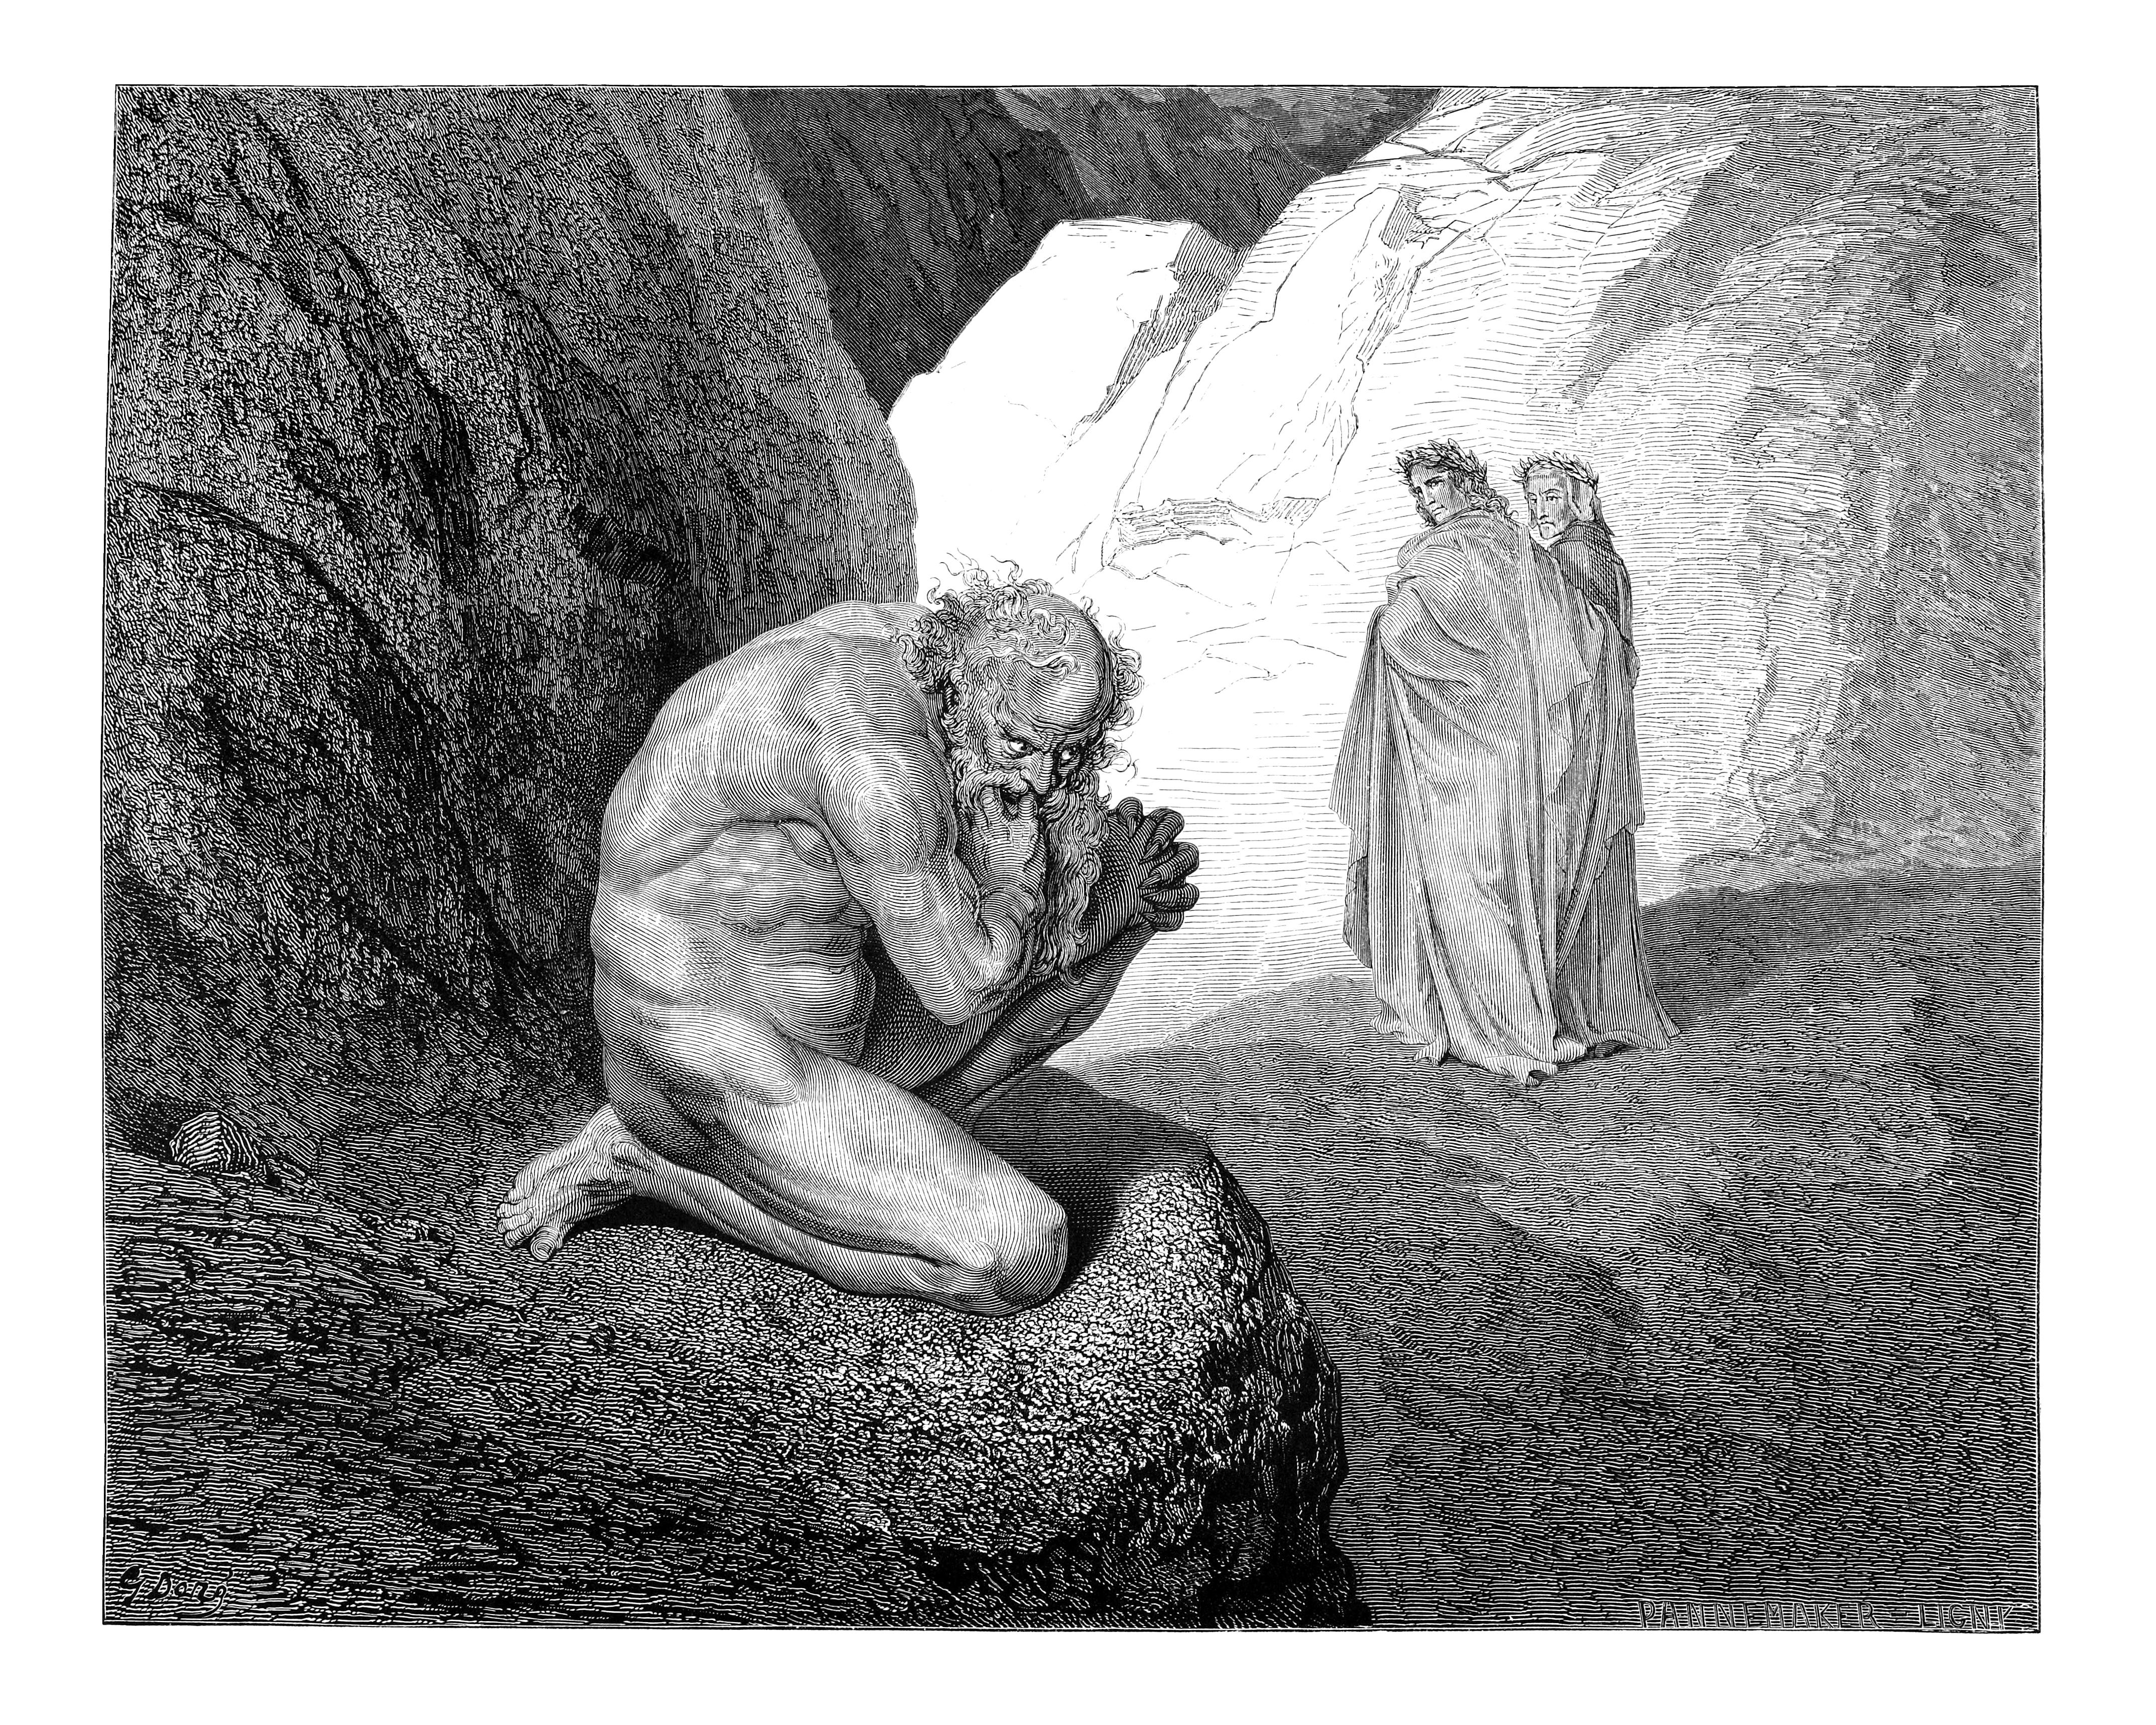
\includegraphics[height=\figsize]{illustrations/book_1/V01, c07(1).jpg}
\end{figure}

\begin{center}
\begin{minipage}{0.8\linewidth}
\textit{\\
"«Pape Satàn, pape Satàn aleppe!»,\\cominci\`o Pluto con la voce chioccia;"} \\
—V01, c07(1) \\~\\
\textit{"\textquotesingle Ah me! O Satan! Satan!\textquotesingle \space loud exclaim'd\\Plutus, in accent hoarse of wild alarm:"} \\
—B01, c07(1)
\end{minipage}
\end{center}

\newpage

\section{Canto 07(2)}

\begin{figure}[ht]
\centering
\includegraphics[height=\figsize]{illustrations/book_1/V01, c07(2).jpg}
\end{figure}

\begin{center}
\begin{minipage}{0.8\linewidth}
\textit{\\
"...d’una parte e d’altra, con grand’urli,\\voltando pesi per forza di poppa."} \\
—V01, c07(2) \\~\\
\textit{"From one side and the other, with loud voice,\\Both roll'd on weights by main forge of their breasts,"} \\
—B01, c07(2)
\end{minipage}
\end{center}

\newpage

\section{Canto 07(3)}

\begin{figure}[ht]
\centering
\includegraphics[height=\figsize]{illustrations/book_1/V01, c07(3).jpg}
\end{figure}

\begin{center}
\begin{minipage}{0.8\linewidth}
\textit{\\
"...io, che di mirare stava inteso,\\vidi genti fangose in quel pantano,\\ignude tutte, con sembiante offeso."} \\
—V01, c07(3) \\~\\
\textit{"...Intent I stood\\To gaze, and in the marish sunk descried\\A miry tribe, all naked, and with looks\\Betok'ning rage. …"} \\
—B01, c07(3)
\end{minipage}
\end{center}

\newpage

\section{Canto 08(1)}

\begin{figure}[ht]
\centering
\includegraphics[height=\figsize]{illustrations/book_1/V01, c08(1).jpg}
\end{figure}

\begin{center}
\begin{minipage}{0.8\linewidth}
\textit{\\
"Tosto che ’l duca e io nel legno fui,\\segando se ne va l’antica prora\\de l’acqua più che non suol con altrui."} \\
—V01, c08(1) \\~\\
\textit{"...Soon as both embark'd,\\Cutting the waves, goes on the ancient prow,\\More deeply than with others it is wont."} \\
—B01, c08(1)
\end{minipage}
\end{center}

\newpage

\section{Canto 08(2)}

\begin{figure}[ht]
\centering
\includegraphics[height=\figsize]{illustrations/book_1/V01, c08(2).jpg}
\end{figure}

\begin{center}
\begin{minipage}{0.8\linewidth}
\textit{\\
"...’l maestro accorto lo sospinse,\\dicendo: «Via costà con li altri cani!»."} \\
—V01, c08(2) \\~\\
\textit{"...my teacher sage\\Aware, thrusting him back: \textquotesingle Away! down there\\To the' other dogs!\textquotesingle..."} \\
—B01, c08(2)
\end{minipage}
\end{center}

\newpage

\section{Canto 08(3)}

\begin{figure}[ht]
\centering
\includegraphics[height=\figsize]{illustrations/book_1/V01, c08(3).jpg}
\end{figure}

\begin{center}
\begin{minipage}{0.8\linewidth}
\textit{\\
"Noi pur giugnemmo dentro a l’alte fosse\\che vallan quella terra sconsolata:"} \\
—V01, c08(3) \\~\\
\textit{"We came within the fosses deep, that moat\\This region comfortless. …"} \\
—B01, c08(3)
\end{minipage}
\end{center}

\newpage

\section{Canto 09(1)}

\begin{figure}[ht]
\centering
\includegraphics[height=\figsize]{illustrations/book_1/V01, c09(1).jpg}
\end{figure}

\begin{center}
\begin{minipage}{0.8\linewidth}
\textit{\\
"...l’occhio m’avea tutto tratto\\ver’ l’alta torre a la cima rovente,\\dove in un punto furon dritte ratto\\tre furie infernal di sangue tinte,"} \\
—V01, c09(1) \\~\\
\textit{"...I beheld uprisen\\At once three hellish furies stain'd with blood:"} \\
—B01, c09(1)
\end{minipage}
\end{center}

\newpage

\section{Canto 09(2)}

\begin{figure}[ht]
\centering
\includegraphics[height=\figsize]{illustrations/book_1/V01, c09(2).jpg}
\end{figure}

\begin{center}
\begin{minipage}{0.8\linewidth}
\textit{\\
"Venne a la porta, e con una verghetta\\l’aperse, che non v’ebbe alcun ritegno."} \\
—V01, c09(2) \\~\\
\textit{"...To the gate\\He came, and with his wand touch'd it, whereat\\Open without impediment it flew."} \\
—B01, c09(2)
\end{minipage}
\end{center}

\newpage

\section{Canto 09(3)}

\begin{figure}[ht]
\centering
\includegraphics[height=\figsize]{illustrations/book_1/V01, c09(3).jpg}
\end{figure}

\begin{center}
\begin{minipage}{0.8\linewidth}
\textit{\\
"...tra gli avelli fiamme erano sparte,\\per le quali eran s\`{\i} del tutto accesi,\\che ferro più non chiede verun’arte."} \\
—V01, c09(3) \\~\\
\textit{"...'midst the graves were scattered flames,\\Wherewith intensely all throughout they burn'd,\\That iron for no craft there hotter needs."} \\
—B01, c09(3)
\end{minipage}
\end{center}

\newpage

\section{Canto 10}

\begin{figure}[ht]
\centering
\includegraphics[height=\figsize]{illustrations/book_1/V01, c10.jpg}
\end{figure}

\begin{center}
\begin{minipage}{0.8\linewidth}
\textit{\\
"...el s’ergea col petto e con la fronte\\com’avesse l’inferno a gran dispitto."} \\
—V01, c10 \\~\\
\textit{"...his breast and forehead there\\Erecting, seem'd as in high scorn he held\\E'en hell. …"} \\
—B01, c10
\end{minipage}
\end{center}

\newpage

\section{Canto 11}

\begin{figure}[ht]
\centering
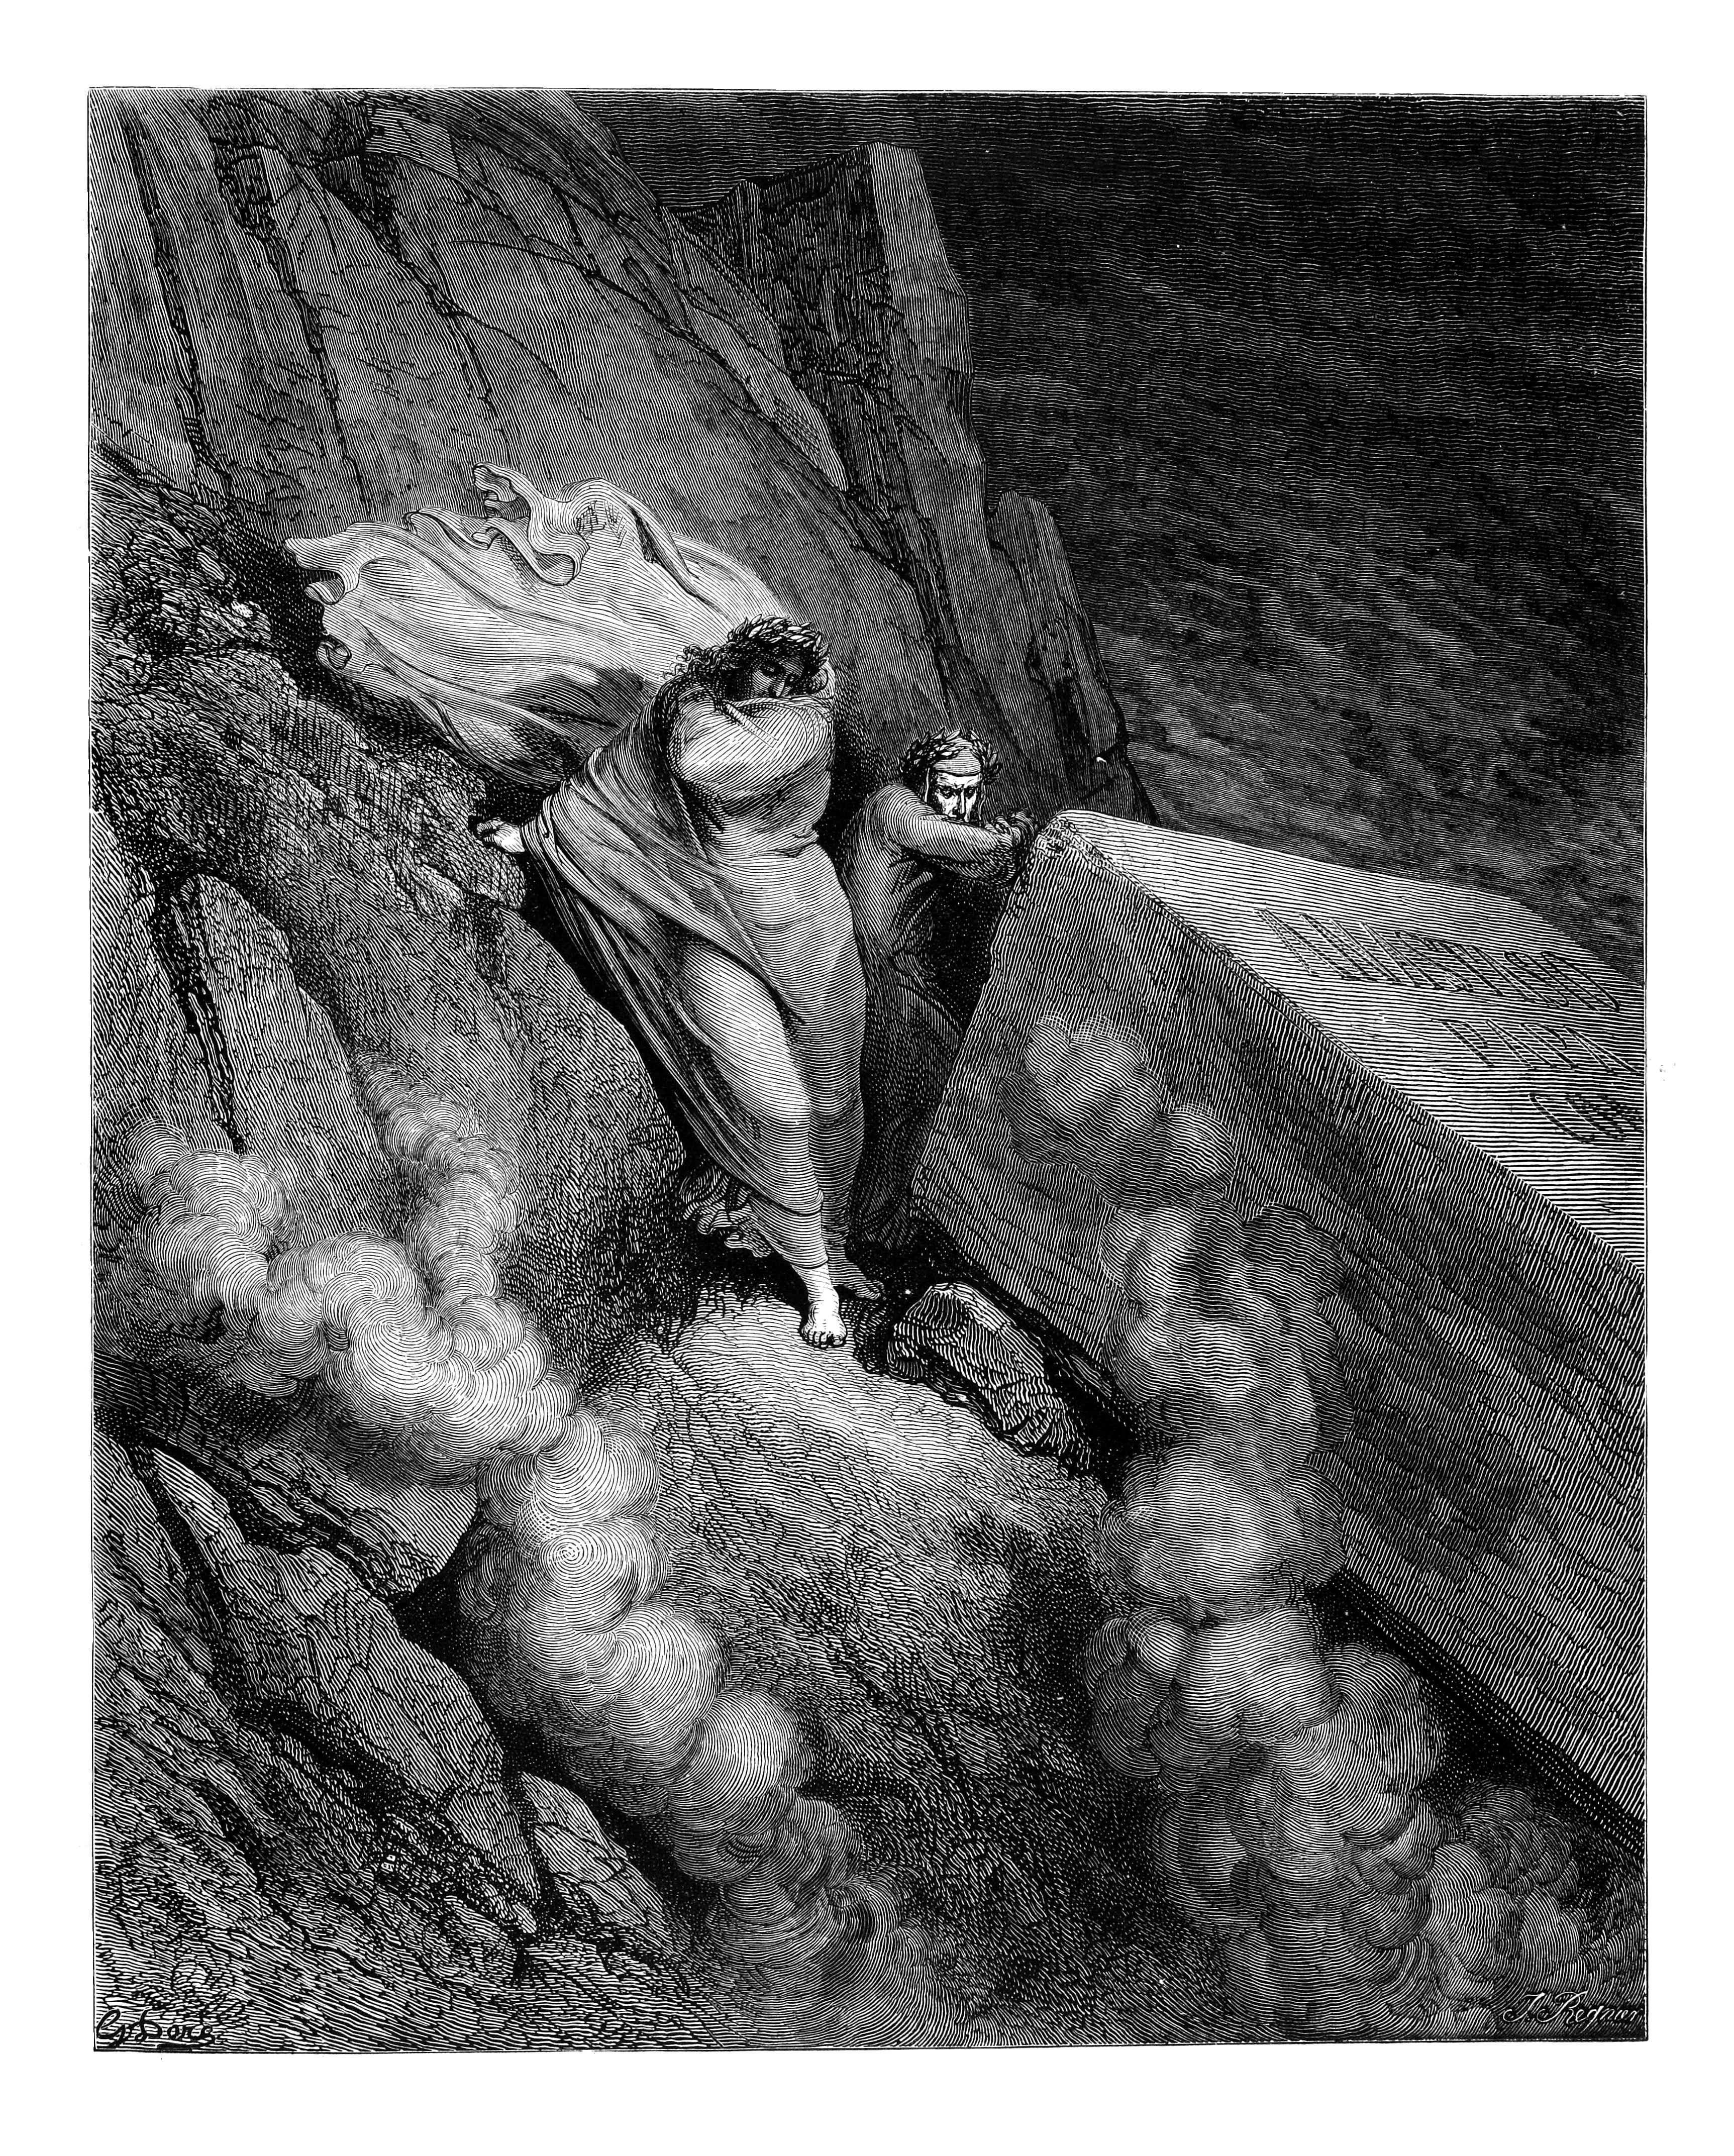
\includegraphics[height=\figsize]{illustrations/book_1/V01, c11.jpg}
\end{figure}

\begin{center}
\begin{minipage}{0.8\linewidth}
\textit{\\
"ci raccostammo, in dietro, ad un coperchio\\d’un grand’avello, …"} \\
—V01, c11 \\~\\
\textit{"...behind the lid\\Of a great monument we stood retir'd,"} \\
—B01, c11
\end{minipage}
\end{center}

\newpage

\section{Canto 12(1)}

\begin{figure}[ht]
\centering
\includegraphics[height=\figsize]{illustrations/book_1/V01, c12(1).jpg}
\end{figure}

\begin{center}
\begin{minipage}{0.8\linewidth}
\textit{\\
"...su la punta de la rotta lacca\\l’infamia di Creti era distesa"} \\
—V01, c12(1) \\~\\
\textit{"At point of the disparted ridge lay stretch'd\\The infamy of Crete, …"} \\
—B01, c12(1)
\end{minipage}
\end{center}

\newpage

\section{Canto 12(2)}

\begin{figure}[ht]
\centering
\includegraphics[height=\figsize]{illustrations/book_1/V01, c12(2).jpg}
\end{figure}

\begin{center}
\begin{minipage}{0.8\linewidth}
\textit{\\
"...in traccia\\corrien centauri, armati di saette,\\come solien nel mondo andare a caccia."} \\
—V01, c12(2) \\~\\
\textit{"On trail ran Centaurs, with keen arrows arm'd,\\As to the chase they on the earth were wont."} \\
—B01, c12(2)
\end{minipage}
\end{center}

\newpage

\section{Canto 12(3)}

\begin{figure}[ht]
\centering
\includegraphics[height=\figsize]{illustrations/book_1/V01, c12(3).jpg}
\end{figure}

\begin{center}
\begin{minipage}{0.8\linewidth}
\textit{\\
"Dintorno al fosso vanno a mille a mille,\\saettando qual anima si svelle\\del sangue…"} \\
—V01, c12(3) \\~\\
\textit{"...Around\\The foss these go by thousands, aiming shafts\\At whatsoever spirit dares emerge"} \\
—B01, c12(3)
\end{minipage}
\end{center}

\newpage

\section{Canto 13(1)}

\begin{figure}[ht]
\centering
\includegraphics[height=\figsize]{illustrations/book_1/V01, c13(1).jpg}
\end{figure}

\begin{center}
\begin{minipage}{0.8\linewidth}
\textit{\\
"Quivi le brutte Arpie lor nidi fanno,"} \\
—V01, c13(1) \\~\\
\textit{"Here the brute Harpies make their nest, …"} \\
—B01, c13(1)
\end{minipage}
\end{center}

\newpage

\section{Canto 13(2)}

\begin{figure}[ht]
\centering
\includegraphics[height=\figsize]{illustrations/book_1/V01, c13(2).jpg}
\end{figure}

\begin{center}
\begin{minipage}{0.8\linewidth}
\textit{\\
"...porsi la mano un poco avante,\\e colsi un ramicel da un gran pruno;"} \\
—V01, c13(2) \\~\\
\textit{"...a little stretching forth my hand,\\From a great wilding gather'd I a branch,"} \\
—B01, c13(2)
\end{minipage}
\end{center}

\newpage

\section{Canto 13(3)}

\begin{figure}[ht]
\centering
\includegraphics[height=\figsize]{illustrations/book_1/V01, c13(3).jpg}
\end{figure}

\begin{center}
\begin{minipage}{0.8\linewidth}
\textit{\\
"...ecco due da la sinistra costa,\\nudi e graffiati, fuggendo sì forte,\\che de la selva rompieno ogni rosta."} \\
—V01, c13(3) \\~\\
\textit{"...lo! there came\\Two naked, torn with briers, in headlong flight,\\That they before them broke each fan o' th' wood."} \\
—B01, c13(3)
\end{minipage}
\end{center}

\newpage

\section{Canto 14}

\begin{figure}[ht]
\centering
\includegraphics[height=\figsize]{illustrations/book_1/V01, c14.jpg}
\end{figure}

\begin{center}
\begin{minipage}{0.8\linewidth}
\textit{\\
"Sovra tutto ’l sabbion, d’un cader lento,\\piovean di foco dilatate falde,"} \\
—V01, c14 \\~\\
\textit{"O'er all the sand fell slowly wafting down\\Dilated flakes of fire, …"} \\
—B01, c14
\end{minipage}
\end{center}

\newpage

\section{Canto 15}

\begin{figure}[ht]
\centering
\includegraphics[height=\figsize]{illustrations/book_1/V01, c15.jpg}
\end{figure}

\begin{center}
\begin{minipage}{0.8\linewidth}
\textit{\\
"fui conosciuto da un, che mi prese\\per lo lembo …"} \\
—V01, c15 \\~\\
\textit{"I was agniz'd of one, who by the skirt\\Caught me, …"} \\
—B01, c15
\end{minipage}
\end{center}

\newpage

\section{Canto 16}

\begin{figure}[ht]
\centering
\includegraphics[height=\figsize]{illustrations/book_1/V01, c16.jpg}
\end{figure}

\begin{center}
\begin{minipage}{0.8\linewidth}
\textit{\\
"...vidi per quell’aere grosso e scuro\\venir notando una figura in suso,\\maravigliosa ad ogne cor sicuro,"} \\
—V01, c16 \\~\\
\textit{"...through the gross and murky air I spied\\A shape come swimming up, that might have quell'd\\The stoutest heart with wonder,"} \\
—B01, c16
\end{minipage}
\end{center}

\newpage

\section{Canto 17}

\begin{figure}[ht]
\centering
\includegraphics[height=\figsize]{illustrations/book_1/V01, c17.jpg}
\end{figure}

\begin{center}
\begin{minipage}{0.8\linewidth}
\textit{\\
"...i’ era\\ne l’aere d’ogne parte, e vidi spenta\\ogne veduta fuor che de la fera."} \\
—V01, c17 \\~\\
\textit{"...round me on each part\\The air I view' d, and other object none\\Save the fell beast. …"} \\
—B01, c17
\end{minipage}
\end{center}

\newpage

\section{Canto 18(1)}

\begin{figure}[ht]
\centering
\includegraphics[height=\figsize]{illustrations/book_1/V01, c18(1).jpg}
\end{figure}

\begin{center}
\begin{minipage}{0.8\linewidth}
\textit{\\
"Di qua, di là, su per lo sasso tetro\\vidi demon cornuti con gran ferze,\\che li battien crudelmente di retro."} \\
—V01, c18(1) \\~\\
\textit{"Each divers way along the grisly rock,\\Horn'd demons I beheld, with lashes huge,\\That on their back unmercifully smote."} \\
—B01, c18(1)
\end{minipage}
\end{center}

\newpage

\section{Canto 18(2)}

\begin{figure}[ht]
\centering
\includegraphics[height=\figsize]{illustrations/book_1/V01, c18(2).jpg}
\end{figure}

\begin{center}
\begin{minipage}{0.8\linewidth}
\textit{\\
"...giù nel fosso\\vidi gente attuffata in uno sterco\\che da li uman privadi parea mosso."} \\
—V01, c18(2) \\~\\
\textit{"...I saw, within the foss below,\\A crowd immers'd in ordure, that appear'd\\Draff of the human body. …"} \\
—B01, c18(2)
\end{minipage}
\end{center}

\newpage

\section{Canto 18(3)}

\begin{figure}[ht]
\centering
\includegraphics[height=\figsize]{illustrations/book_1/V01, c18(3).jpg}
\end{figure}

\begin{center}
\begin{minipage}{0.8\linewidth}
\textit{\\
"Taide è, la puttana …"} \\
—V01, c18(3) \\~\\
\textit{"Thais is this, the harlot, …"} \\
—B01, c18(3)
\end{minipage}
\end{center}

\newpage

\section{Canto 19}

\begin{figure}[ht]
\centering
\includegraphics[height=\figsize]{illustrations/book_1/V01, c19.jpg}
\end{figure}

\begin{center}
\begin{minipage}{0.8\linewidth}
\textit{\\
"...mentr’io li cantava cotai note,\\o ira o coscienza che ’l mordesse,\\forte spingava con ambo le piote. …"} \\
—V01, c19 \\~\\
\textit{"...as thus I sung, he, whether wrath\\Or conscience smote him, violent upsprang\\Spinning on either sole. …"} \\
—B01, c19
\end{minipage}
\end{center}

\newpage

\section{Canto 21(1)}

\begin{figure}[ht]
\centering
\includegraphics[height=\figsize]{illustrations/book_1/V01, c21(1).jpg}
\end{figure}

\begin{center}
\begin{minipage}{0.8\linewidth}
\textit{\\
"Non altrimenti i cuoci a’ lor vassalli\\fanno attuffare in mezzo la caldaia\\la carne con li uncin, …"} \\
—V01, c21(1) \\~\\
\textit{"E'en thus the cook bestirs him, with his grooms,\\To thrust the flesh into the caldron down\\With flesh-hooks, …"} \\
—B01, c21(1)
\end{minipage}
\end{center}

\newpage

\section{Canto 21(2)}

\begin{figure}[ht]
\centering
\includegraphics[height=\figsize]{illustrations/book_1/V01, c21(2).jpg}
\end{figure}

\begin{center}
\begin{minipage}{0.8\linewidth}
\textit{\\
"«Nessun di voi sia fello! …"} \\
—V01, c21(2) \\~\\
\textit{"Be none of you outrageous: …"} \\
—B01, c21(2)
\end{minipage}
\end{center}

\newpage

\section{Canto 22(1)}

\begin{figure}[ht]
\centering
\includegraphics[height=\figsize]{illustrations/book_1/V01, c22(1).jpg}
\end{figure}

\begin{center}
\begin{minipage}{0.8\linewidth}
\textit{\\
"Lo Navarrese ben suo tempo colse;"} \\
—V01, c22(1) \\~\\
\textit{"The spirit of Navarre chose well his time,"} \\
—B01, c22(1)
\end{minipage}
\end{center}

\newpage

\section{Canto 22(2)}

\begin{figure}[ht]
\centering
\includegraphics[height=\figsize]{illustrations/book_1/V01, c22(2).jpg}
\end{figure}

\begin{center}
\begin{minipage}{0.8\linewidth}
\textit{\\
"...volse li artigli al suo compagno,\\e fu con lui sopra ’l fosso ghermito."} \\
—V01, c22(2) \\~\\
\textit{"...O'er the dyke\\In grapple close they join'd; …"} \\
—B01, c22(2)
\end{minipage}
\end{center}

\newpage

\section{Canto 23(1)}

\begin{figure}[ht]
\centering
\includegraphics[height=\figsize]{illustrations/book_1/V01, c23(1).jpg}
\end{figure}

\begin{center}
\begin{minipage}{0.8\linewidth}
\textit{\\
"...l’alta provedenza che lor volle\\porre ministri de la fossa quinta,\\poder di partirs’indi a tutti tolle."} \\
—V01, c23(1) \\~\\
\textit{"...that high Providence,\\Which plac'd them ministers of the fifth foss,\\Power of departing thence took from them all."} \\
—B01, c23(1)
\end{minipage}
\end{center}

\newpage

\section{Canto 23(2)}

\begin{figure}[ht]
\centering
\includegraphics[height=\figsize]{illustrations/book_1/V01, c23(2).jpg}
\end{figure}

\begin{center}
\begin{minipage}{0.8\linewidth}
\textit{\\
"Elli avean cappe con cappucci bassi\\dinanzi a li occhi, …"} \\
—V01, c23(2) \\~\\
\textit{"Caps had they on, with hoods, that fell low down\\Before their eyes, ..."} \\
—B01, c23(2)
\end{minipage}
\end{center}

\newpage

\section{Canto 23(3)}

\begin{figure}[ht]
\centering
\includegraphics[height=\figsize]{illustrations/book_1/V01, c23(3).jpg}
\end{figure}

\begin{center}
\begin{minipage}{0.8\linewidth}
\textit{\\
"...a l’occhio mi corse\\un, crucifisso in terra con tre pali."} \\
—V01, c23(3) \\~\\
\textit{"...one had caught my eye,\\Fix' d to a cross with three stakes on the ground:"} \\
—B01, c23(3)
\end{minipage}
\end{center}

\newpage

\section{Canto 24}

\begin{figure}[ht]
\centering
\includegraphics[height=\figsize]{illustrations/book_1/V01, c24.jpg}
\end{figure}

\begin{center}
\begin{minipage}{0.8\linewidth}
\textit{\\
"...vidivi entro terribile stipa\\di serpenti, …"} \\
—V01, c24 \\~\\
\textit{"...I saw a crowd within\\Of serpents terrible, ..."} \\
—B01, c24
\end{minipage}
\end{center}

\newpage

\section{Canto 25}

\begin{figure}[ht]
\centering
\includegraphics[height=\figsize]{illustrations/book_1/V01, c25.jpg}
\end{figure}

\begin{center}
\begin{minipage}{0.8\linewidth}
\textit{\\
"...un serpente con sei piè si lancia\\dinanzi a l’uno, e tutto a lui s’appiglia."} \\
—V01, c25 \\~\\
\textit{"...lo! a serpent with six feet\\Springs forth on one, and fastens full upon him:"} \\
—B01, c25
\end{minipage}
\end{center}

\newpage

\section{Canto 26}

\begin{figure}[ht]
\centering
\includegraphics[height=\figsize]{illustrations/book_1/V01, c26.jpg}
\end{figure}

\begin{center}
\begin{minipage}{0.8\linewidth}
\textit{\\
"...«Dentro dai fuochi son li spirti;\\catun si fascia di quel ch’elli è inceso»."} \\
—V01, c26 \\~\\
\textit{"Within these ardours are the spirits, each\\Swath'd in confining fire.\textquotesingle…"} \\
—B01, c26
\end{minipage}
\end{center}

\newpage

\section{Canto 28(1)}

\begin{figure}[ht]
\centering
\includegraphics[height=\figsize]{illustrations/book_1/V01, c28(1).jpg}
\end{figure}

\begin{center}
\begin{minipage}{0.8\linewidth}
\textit{\\
"guardommi, e con le man s’aperse il petto,\\dicendo: «Or vedi com’io mi dilacco!"} \\
—V01, c28(1) \\~\\
\textit{"He ey'd me, with his hands laid his breast bare,\\And cried; \textquotesingle Now mark how I do rip me! …"} \\
—B01, c28(1)
\end{minipage}
\end{center}

\newpage

\section{Canto 28(2)}

\begin{figure}[ht]
\centering
\includegraphics[height=\figsize]{illustrations/book_1/V01, c28(2).jpg}
\end{figure}

\begin{center}
\begin{minipage}{0.8\linewidth}
\textit{\\
"Oh quanto mi pareva sbigottito\\con la lingua tagliata ne la strozza\\Curio, ch’a dir fu così ardito!"} \\
—V01, c28(2) \\~\\
\textit{"...Oh how terrified\\Methought was Curio, from whose throat was cut\\The tongue, which spake that hardy word. …"} \\
—B01, c28(2)
\end{minipage}
\end{center}

\newpage

\section{Canto 28(3)}

\begin{figure}[ht]
\centering
\includegraphics[height=\figsize]{illustrations/book_1/V01, c28(3).jpg}
\end{figure}

\begin{center}
\begin{minipage}{0.8\linewidth}
\textit{\\
"...’l capo tronco tenea per le chiome,\\pesol con mano a guisa di lanterna;\\e quel mirava noi e dicea: «Oh me!»."} \\
—V01, c28(3) \\~\\
\textit{"...By the hair\\It bore the sever'd member, lantern-wise\\Pendent in hand, which look'd at us and said,\\ \textquotesingle Woe's me!\textquotesingle…"} \\
—B01, c28(3)
\end{minipage}
\end{center}

\newpage

\section{Canto 29(1)}

\begin{figure}[ht]
\centering
\includegraphics[height=\figsize]{illustrations/book_1/V01, c29(1).jpg}
\end{figure}

\begin{center}
\begin{minipage}{0.8\linewidth}
\textit{\\
"La molta gente e le diverse piaghe\\avean le luci mie s\`{\i} inebriate,\\che de lo stare a piangere eran vaghe."} \\
—V01, c29(1) \\~\\
\textit{"So were mine eyes inebriate with view\\Of the vast multitude, whom various wounds\\Disfigur'd, that they long'd to stay and weep."} \\
—B01, c29(1)
\end{minipage}
\end{center}

\newpage

\section{Canto 29(2)}

\begin{figure}[ht]
\centering
\includegraphics[height=\figsize]{illustrations/book_1/V01, c29(2).jpg}
\end{figure}

\begin{center}
\begin{minipage}{0.8\linewidth}
\textit{\\
"...lo fondo, la ’ve la ministra\\de l’alto Sire infallibil giustizia\\punisce i falsador…"} \\
—V01, c29(2) \\~\\
\textit{"...the depth, wherein\\The minister of the most mighty Lord,\\All-searching Justice, dooms to punishment\\The forgers..."} \\
—B01, c29(2)
\end{minipage}
\end{center}

\newpage

\section{Canto 29(3)}

\begin{figure}[ht]
\centering
\includegraphics[height=\figsize]{illustrations/book_1/V01, c29(3).jpg}
\end{figure}

\begin{center}
\begin{minipage}{0.8\linewidth}
\textit{\\
"Io vidi due sedere a sé poggiati,\\com’a scaldar si poggia tegghia a tegghia,"} \\
—V01, c29(3) \\~\\
\textit{"...two I mark'd, that sat\\Propp'd 'gainst each other, as two brazen pans\\Set to retain the heat. …"} \\
—B01, c29(3)
\end{minipage}
\end{center}

\newpage

\section{Canto 30(1)}

\begin{figure}[ht]
\centering
\includegraphics[height=\figsize]{illustrations/book_1/V01, c30(1).jpg}
\end{figure}

\begin{center}
\begin{minipage}{0.8\linewidth}
\textit{\\
"...io vidi in due ombre smorte e nude,\\che mordendo correvan…"} \\
—V01, c30(1) \\~\\
\textit{"...two pale and naked ghost I saw\\That gnarling wildly scamper'd, …"} \\
—B01, c30(1)
\end{minipage}
\end{center}

\newpage

\section{Canto 30(2)}

\begin{figure}[ht]
\centering
\includegraphics[height=\figsize]{illustrations/book_1/V01, c30(2).jpg}
\end{figure}

\begin{center}
\begin{minipage}{0.8\linewidth}
\textit{\\
"...«Quell’è l’anima antica\\di Mirra scellerata, …"} \\
—V01, c30(2) \\~\\
\textit{"...\textquotesingle That is the ancient soul\\Of wretched Myrrha,\textquotesingle…"} \\
—B01, c30(2)
\end{minipage}
\end{center}

\newpage

\section{Canto 31(1)}

\begin{figure}[ht]
\centering
\includegraphics[height=\figsize]{illustrations/book_1/V01, c31(1).jpg}
\end{figure}

\begin{center}
\begin{minipage}{0.8\linewidth}
\textit{\\
"questi è Nembrotto per lo cui mal coto\\pur un linguaggio nel mondo non s’usa."} \\
—V01, c31(1) \\~\\
\textit{"...Nimrod is this,\\Through whose ill counsel in the world no more\\One tongue prevails. …"} \\
—B01, c31(1)
\end{minipage}
\end{center}

\newpage

\section{Canto 31(2)}

\begin{figure}[ht]
\centering
\includegraphics[height=\figsize]{illustrations/book_1/V01, c31(2).jpg}
\end{figure}

\begin{center}
\begin{minipage}{0.8\linewidth}
\textit{\\
"«Questo superbo volle esser esperto\\di sua potenza contra ’l sommo Giove»,"} \\
—V01, c31(2) \\~\\
\textit{"...\textquotesingle This proud one\\Would of his strength against almighty Jove\\Make trial,\textquotesingle…"} \\
—B01, c31(2)
\end{minipage}
\end{center}

\newpage

\section{Canto 31(3)}

\begin{figure}[ht]
\centering
\includegraphics[height=\figsize]{illustrations/book_1/V01, c31(3).jpg}
\end{figure}

\begin{center}
\begin{minipage}{0.8\linewidth}
\textit{\\
"Ma lievemente al fondo che divora\\Lucifero con Giuda, ci spos\`o;"} \\
—V01, c31(3) \\~\\
\textit{"...in th' abyss,\\That Lucifer with Judas low ingulfs,\\lightly he plac'd us; …"} \\
—B01, c31(3)
\end{minipage}
\end{center}

\newpage

\section{Canto 32(1)}

\begin{figure}[ht]
\centering
\includegraphics[height=\figsize]{illustrations/book_1/V01, c32(1).jpg}
\end{figure}

\begin{center}
\begin{minipage}{0.8\linewidth}
\textit{\\
"...insin là dove appar vergogna\\eran l’ombre dolenti ne la ghiaccia,"} \\
—V01, c32(1) \\~\\
\textit{"...to where modest shame appears, thus low\\Blue pinch'd and shrin'd in ice the spirits stood,"} \\
—B01, c32(1)
\end{minipage}
\end{center}

\newpage

\section{Canto 32(2)}

\begin{figure}[ht]
\centering
\includegraphics[height=\figsize]{illustrations/book_1/V01, c32(2).jpg}
\end{figure}

\begin{center}
\begin{minipage}{0.8\linewidth}
\textit{\\
"...lo presi per la cuticagna,\\e dissi: «El converrà che tu ti nomi,\\o che capel qui sù non ti rimagna»."} \\
—V01, c32(2) \\~\\
\textit{"...seizing on his hinder scalp, I cried:\\ \textquotesingle Name thee, or not a hair shall tarry here.\textquotesingle"} \\
—B01, c32(2)
\end{minipage}
\end{center}

\newpage

\section{Canto 32(3)}

\begin{figure}[ht]
\centering
\includegraphics[height=\figsize]{illustrations/book_1/V01, c32(3).jpg}
\end{figure}

\begin{center}
\begin{minipage}{0.8\linewidth}
\textit{\\
"...io vidi due ghiacciati in una buca,\\s\`{\i} che l’un capo a l’altro era cappello;"} \\
—V01, c32(3) \\~\\
\textit{"...I beheld two spirits by the ice\\Pent in one hollow, that the head of one\\Was cowl unto the other; …"} \\
—B01, c32(3)
\end{minipage}
\end{center}

\newpage

\section{Canto 33(1)}

\begin{figure}[ht]
\centering
\includegraphics[height=\figsize]{illustrations/book_1/V01, c33(1).jpg}
\end{figure}

\begin{center}
\begin{minipage}{0.8\linewidth}
\textit{\\
"...un poco di raggio si fu messo\\nel doloroso carcere, e io scorsi\\per quattro visi il mio aspetto stesso,"} \\
—V01, c33(1) \\~\\
\textit{"...a faint beam\\Had to our doleful prison made its way,\\And in four countenances I descry'd\\The image of my own, …"} \\
—B01, c33(1)
\end{minipage}
\end{center}

\newpage

\section{Canto 33(2)}

\begin{figure}[ht]
\centering
\includegraphics[height=\figsize]{illustrations/book_1/V01, c33(2).jpg}
\end{figure}

\begin{center}
\begin{minipage}{0.8\linewidth}
\textit{\\
"Gaddo mi si gittò disteso a’ piedi,\\dicendo: «Padre mio, ché non mi aiuti?»."} \\
—V01, c33(2) \\~\\
\textit{"...Geddo at my feet\\Outstretch'd did fling him, crying, \textquotesingle Hast no help\\For me, my father!\textquotesingle..."} \\
—B01, c33(2)
\end{minipage}
\end{center}

\newpage

\section{Canto 33(3)}

\begin{figure}[ht]
\centering
\includegraphics[height=\figsize]{illustrations/book_1/V01, c33(3).jpg}
\end{figure}

\begin{center}
\begin{minipage}{0.8\linewidth}
\textit{\\
"...come tu mi vedi,\\vid’io cascar li tre ad uno ad uno\\tra ’l quinto dì e ’l sesto; …"} \\
—V01, c33(3) \\~\\
\textit{"Plainly as thou seest me, saw I the three\\Fall one by one 'twixt the fifth day and sixth:"} \\
—B01, c33(3)
\end{minipage}
\end{center}

\newpage

\section{Canto 34(1)}

\begin{figure}[ht]
\centering
\includegraphics[height=\figsize]{illustrations/book_1/V01, c34(1).jpg}
\end{figure}

\begin{center}
\begin{minipage}{0.8\linewidth}
\textit{\\
"...ecco il loco\\ove convien che di fortezza t’armi»."} \\
—V01, c34(1) \\~\\
\textit{"…lo the place,\\Where thou hast need to arm thy heart with strength.\textquotesingle"} \\
—B01, c34(1)
\end{minipage}
\end{center}

\newpage

\section{Canto 34(2)}

\begin{figure}[ht]
\centering
\includegraphics[height=\figsize]{illustrations/book_1/V01, c34(2).jpg}
\end{figure}

\begin{center}
\begin{minipage}{0.8\linewidth}
\textit{\\
"Lo duca e io per quel cammino ascoso\\intrammo a ritornar nel chiaro mondo;"} \\
—V01, c34(2) \\~\\
\textit{"...By that hidden way\\My guide and I did enter, to return\\To the fair world: …"} \\
—B01, c34(2)
\end{minipage}
\end{center}

\newpage

\section{Canto 34(3)}

\begin{figure}[ht]
\centering
\includegraphics[height=\figsize]{illustrations/book_1/V01, c34(3).jpg}
\end{figure}

\begin{center}
\begin{minipage}{0.8\linewidth}
\textit{\\
"...quindi uscimmo a riveder le stelle."} \\
—V01, c34(3) \\~\\
\textit{"Thus issuing we again beheld the stars."} \\
—B01, c34(3)
\end{minipage}
\end{center}

\end{document}